\documentclass[12pt]{article}
\usepackage{amsmath}
\usepackage{graphicx} % Required for inserting images
\usepackage{array}
\usepackage{pgfplots}
\usepackage{float}
\usepackage{tikz}
\usetikzlibrary{mindmap}
\usepackage[top=2.75cm, bottom=2.55cm, left=2.5cm, right=2.5cm]{geometry}
\usepackage{enumitem}
\title{}
\author{Shreyash Bhilwade 2021EE30178}
\date{December 2023}

\begin{document}
\maketitle
\newpage
\tableofcontents
\newpage
\section{Research Question}

\begin{figure}
  \centering
  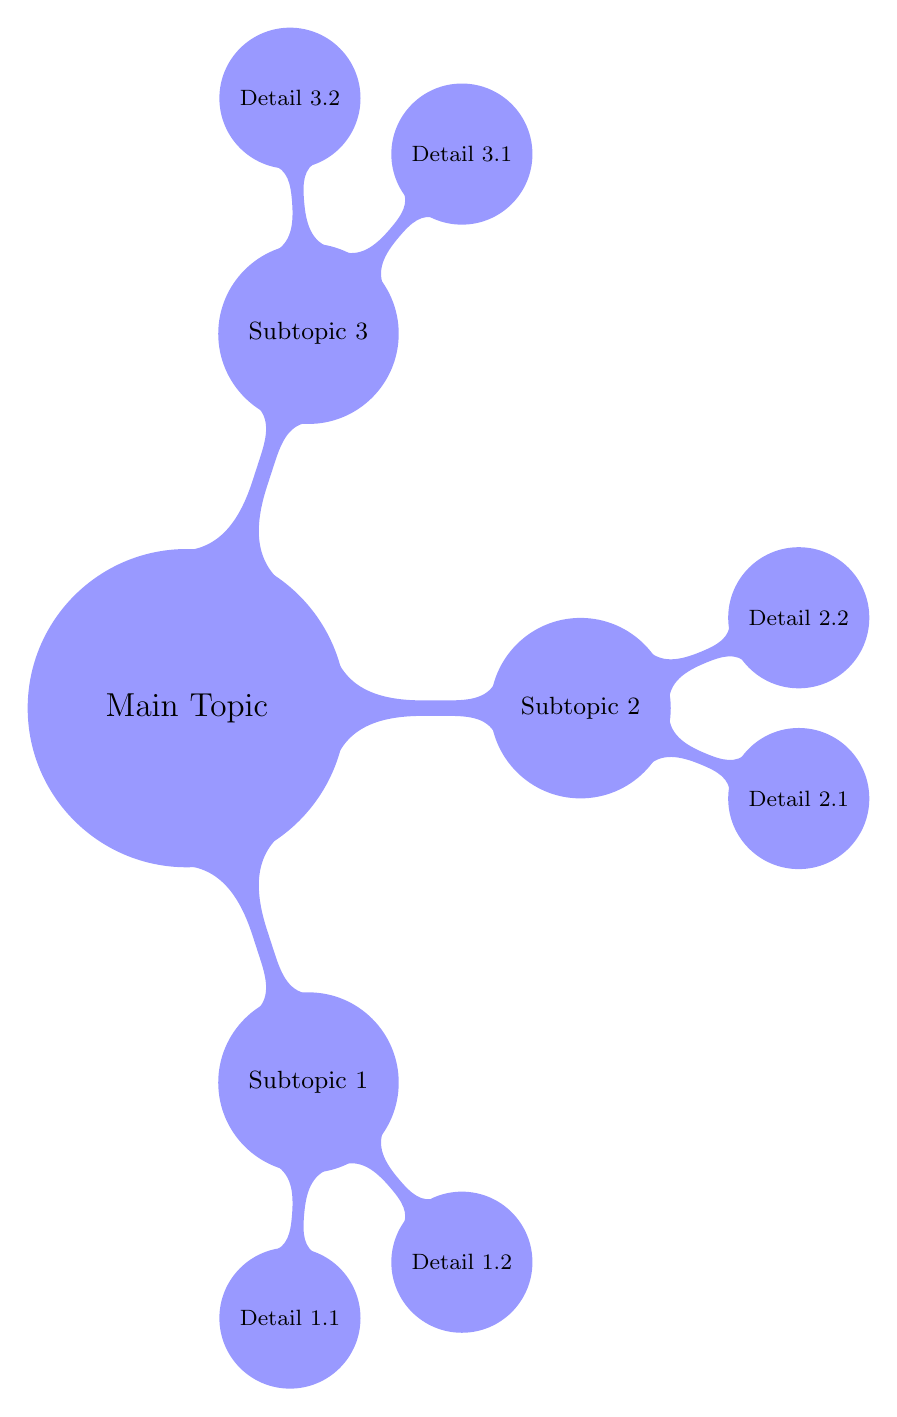
\begin{tikzpicture}[mindmap, grow cyclic, every node/.style=concept, concept color=blue!40,
    level 1/.append style={level distance=5cm,sibling angle=72},
    level 2/.append style={level distance=3cm,sibling angle=45}]

    \node {Main Topic}
      child { node {Subtopic 1}
        child { node {Detail 1.1} }
        child { node {Detail 1.2} }
      }
      child { node {Subtopic 2}
        child { node {Detail 2.1} }
        child { node {Detail 2.2} }
      }
      child { node {Subtopic 3}
        child { node {Detail 3.1} }
        child { node {Detail 3.2} }
      };
  \end{tikzpicture}
  \caption{Mind Map Example}
\end{figure}

\end{document}
